\documentclass[letterpaper]{article}
% ====
% BASIC PACKAGES
% ====
\usepackage{hyperref}
\usepackage{graphicx}
\usepackage{todonotes}
\usepackage{marginnote}
\usepackage[margin=1.5in]{geometry}

% Hide page number when page is empty
% \usepackage{empheq}
% \usepackage{breqn}

% Math stuff
\usepackage{amsmath, amsfonts, bbold}
\usepackage{physics}
\usepackage[nomessages]{fp} % Doing arithmetic in latex using, e.g., \FPeval

\usepackage{mathrsfs} % Fancy script capitals
\usepackage{cancel}
\usepackage{bm} % bold maths
\usepackage{enumitem}

% ====
% Styling 
% ====

% Changes footnote markers to symbols (dagger, double dagger, etc.)
% \usepackage[symbol]{footmisc} 

% Equation numbering by section, subsection.
\numberwithin{equation}{section} % this command comes from amsmath
% \renewcommand{\theequation}{\arabic{section}.\arabic{equation}} 

% New paragraphs aren't indented.
\usepackage{parskip}
\setlength{\parskip}{3ex}

% ----
% Colours
% ----
\usepackage{xcolor, soul}
\definecolor{correct}{HTML}{009900}
\DeclareMathSymbol{\shortminus}{\mathbin}{AMSa}{"39}

\definecolor{lblue}{RGB}{102,204,255}
\colorlet{soulblue}{lblue!30}
\sethlcolor{soulblue}

% ----
% Section headers
% -----
\usepackage{sectsty}
\usepackage[scaled=.92]{helvet}

\sectionfont{\fontfamily{phv}\selectfont}
\subsectionfont{\fontfamily{phv}\selectfont}
\usepackage{titlesec}
\titlespacing*{\subsection}
{0px}{0px}{0.5ex}
\titlespacing{\subsection}
{0pt}{0.25ex}{0.5ex}

%make margin notes on left side and make the font size the same as footnote
\renewcommand*{\marginfont}{\footnotesize}
\renewcommand*{\raggedleftmarginnote}{\flushleft}



% ----
% Page headers using fancyhdr
% ----
\usepackage{fancyhdr}
\pagestyle{fancy}
\fancyhead[L]{\fontfamily{phv}\selectfont NEUTRON STAR COOLING}
\fancyhead[C]{}
\fancyhead[R]{\thepage}
\fancyfoot[L,R,C]{}

\setlength{\headheight}{14pt}

% ====
% Custom environments
% ====

% ----
% Blue boxes!
% ----
\usepackage{mdframed}
\mdfsetup{skipabove=0pt,skipbelow=3pt}
\global\mdfdefinestyle{blue}{
    topline=false, 
    rightline=false,
    bottomline=false,
    linecolor=lblue!85!white, 
    linewidth=2.5pt,
    subtitlebackgroundcolor=lblue!30!white,
    backgroundcolor=lblue!30!white,
    skipabove=10pt,skipbelow=10pt
}

\usepackage{caption} % to add captions to figures inside mdframed environment


% Bold script maths variables
\DeclareMathAlphabet{\mathscrbf}{OMS}{mdugm}{b}{n}
\newcommand{\Jscr}{\mathscr{J}}
\newcommand{\Jscrb}{\mathscr{J}}

\newenvironment{bluenv}[1]
    {\begin{mdframed}[style=blue, frametitle=#1]}
    {\end{mdframed}}

% monospace 
\def\code#1{\texttt{#1}}

% \makeatother
% ----
% Problem/solution environments
% ----
\newmdenv[
    topline=false, 
    rightline=false,
    bottomline=false,
    leftline=false,
    innertopmargin=5pt,
    innerleftmargin=0pt,
    innerrightmargin=0pt,
    innerbottommargin=10pt,
    backgroundcolor=white,
    frametitle=Solution,
    frametitlefont=\normalfont\itshape]
    {solution}

\newmdenv[style=blue,backgroundcolor=lblue!20!white]{problem}

% \renewcommand{\theenumi}{\alph{enumi}}
% \renewcommand{\labelenumi}{(\theenumi)}
% \renewcommand{\theenumii}{\roman{enumii}}
% \renewcommand{\labelenumii}{(\theenumii)}

%====
% MACROS
%====

% -----
% References
% -----
% Equations
\newcommand{\eref}[1]{eq.~(\ref{#1})}
\newcommand{\Eref}[1]{Eq.~(\ref{#1})}

% Sections
\newcommand{\sref}[1]{sec.~(\ref{#1})}
\newcommand{\Sref}[1]{Sec.~(\ref{#1})}

% Figures
\newcommand{\fref}[1]{fig.~(\ref{#1})}
\newcommand{\Fref}[1]{Fig.~(\ref{#1})}

% Appendices
\newcommand{\appref}[1]{appendix~\ref{#1}}
\newcommand{\Appref}[1]{Appendix~\ref{#1}}
% -----
% Subsections, environments
% -----

% Subsection command so I don't have to adjust the leading whitespace every time. There is definitely a better way to do this...
\newcommand{\subsec}[1]{%
    \vspace{7px}
    \subsection{#1}
}

% ----
% Physics
% ----
\newcommand*{\pvec}[1][]{\ensuremath{\bm{p}_{#1}}}
\newcommand*{\pmag}[1][]{\ensuremath{|\bm{p}_{#1}|}}


% ----
% Labels 
% ----
% Number any equation.
\newcommand\numberthis{\addtocounter{equation}{1}\tag{\theequation}}

% ----
% Macros specific to this project
% ----
\newcommand{\Qvec}[1]{\bm{Q}_{#1}}
\newcommand{\Qmag}[1]{|\bm{Q}_{#1}|}

\author{Ray Hagimoto}  
\date{\today}
\title{Neutron star cooling by axion emission}

\begin{document}
    \maketitle
    \tableofcontents
    \newpage
    % start notes
    %===
% SECTION: Introduction
%===
\section{Introduction}
\label{sec:introduction}
The goal of this project is to evaluate the integral 

%---
% emissivity integral
%---
\begin{bluenv}{Emissivity integral}
    \begin{equation}
    \label{eq:emissivity-integral}
    \begin{aligned}
        \varepsilon_{3'} = \int 
            & f_1 f_2 (1 - f_{1'}) (1 - f_{2'}) (1 + f_{3'}) \\
            &\times E_{3'} \,
            \sum_{\sigma, \sigma'} | \mathcal{M} |^2 \,
            \dd \Phi_3 \big( (p_1 + p_2)^2; 1', 2', 3'\big)
            \,
            \frac{\dd^3 p_1}{(2\pi)^3\,2 E_1}
            \frac{\dd^3 p_2}{(2\pi)^3\,2 E_2} 
            \; 
    \end{aligned}
    \end{equation}
\end{bluenv}
where, 
\begin{bluenv}{Lorentz invariant phase space measure}
    \begin{equation}
        \label{eq:LIPS}
        \dd \Phi_n \big((p_a + p_b)^2; 1, \ldots, n \big) \equiv 
        \prod_{i=1}^{n}
        \bigg[
             \delta (p_i^2 - m_i^2) \, \Theta(p_i^0) \, 
            \frac{\dd^4 p_i}{(2\pi)^3}
        \bigg] \, (2\pi)^4 \delta^4 
        \bigg( 
            p_a + p_b - \sum_{i=1}^{n} p_i
        \bigg) \quad 
    \end{equation}
\end{bluenv}
is the Lorentz-invariant phase space measure, and
\begin{equation*}
    f_i \equiv f_{FD}(E_i) \equiv \frac{1}{e^{(E_i - \mu_i)/T} + 1}
\end{equation*}
is the Fermi-Dirac distribution. 
The spin-summed matrix element squared is given by
\begin{bluenv}{Spin-summed matrix element}
    \begin{equation}
        \label{eq:matrix-element}
        \sum_{\sigma, \sigma'} | \mathcal{M} |^2 
            = 
            \frac{128 \, g^2_{ae\mu} e^4}{(m_1^2 - m_{1'}^2)^2} \,
            \frac{
                 (p_1 \cdot p_{1'} - m_1 m_{1'})
                (p_2 \cdot p_{3'})
                (p_{2'} \cdot p_{3'})
            }
            {
                (p_2 - p_{2'})^4
            } \; \, .
    \end{equation}
\end{bluenv}


%====
% SUBSECTION: Direct integration
%====
\subsec{Integration in terms of momentum variables (didn't work)}
\label{subsec:direct-momentum-integration}
\emph{The first strategy I used to evaluate this integral was to do the integration directly in terms of the momentum variables. Below are the notes I wrote detailing my strategy.}

We can use the momentum conserving Dirac delta to evaluate the $\bm{p}_{2'}$ integral, setting
\begin{align}
    \bm{p}_{2'} = \bm{p}_{1} + \bm{p}_{2} - \bm{p}_{1'} - \bm{p}_{3'}.
\end{align}
We now choose to align the $z$-axis with $\bm{p}_1$ and measure angles with respect to this axis. 
Converting to spherical polar coordinates gives, for example, $\dd^3 p_{3'} = p_{3'}^2 \, \dd p_{3'} \, \dd \cos \theta_{13'} \, \dd \phi_{13'}$
\footnote{The angle $\phi_{13'}$ is not measured with respect to $\bm{p}_1$, it is measured to some axis orthogonal to $\bm{p}_1$. We don't need to define that axis explicitly as long as the other angles $\phi_{1i}$ are measured with respect to the same axis.}
. 
Then the energy conserving Dirac delta can be used to evaluate the $\dd p_{3'}$ integral in the following way. 
First, we use $E = \sqrt{p^2 + m^2}$ to rewrite the masses. 
Then we use momentum conservation to make the replacement $\bm{p}_{2'} \rightarrow \bm{p}_{1} + \bm{p}_{2} - \bm{p}_{1'} - \bm{p}_{3'}$:
\begin{align*}
    &E_1 + E_2 
    = E_{1'} + E_{2'} + E_{3'}\\
    &\Rightarrow \sqrt{p_1^2 + m_1^2} + \sqrt{p_{2}^2 + m_2^2} =
        \sqrt{p_{1'}^2 + m_{1'}^2} + 
        \sqrt{p_{2'}^2 + m_{2'}^2} + 
        \sqrt{p_{3'}^2 + m_{3'}^2}\\
    &\Rightarrow \sqrt{p_1^2 + m_1^2} + \sqrt{p_{2}^2 + m_2^2} =
        \sqrt{p_{1'}^2 + m_{1'}^2} + 
        \sqrt{(\bm{p}_{1} + \bm{p}_{2} - \bm{p}_{1'} - \bm{p}_{3'})^2 + m_{2'}^2} + 
        \sqrt{p_{3'}^2 + m_{3'}^2}. \numberthis{} \label{eq:p3p-equation-1}
\end{align*} 
We would like to solve eqn. (\ref{eq:p3p-equation-1}) for $p_{3'}$, but there is a problem coming from the fact that $p_{3'}$ appears under two square root symbols which makes it impossible to get an expression of the form $p_{3'} = \cdots$. 
Instead, we will make the approximation that because $p_{3'} \ll p_{i}$ for $i \in \{1, 2, 1', 2'\}$ that we can ignore the $p_{3'}$ that shows up in $\sqrt{(\bm{p}_{1} + \bm{p}_{2} - \bm{p}_{1'} - \bm{p}_{3'})^2 + m_{2'}^2}$~. 
The result we obtain when solving for $p_{3'}$ is then
\begin{equation}
\begin{aligned}
    p_{3'} = 
        \bigg[
            &m_1^2 + m_{1'}^2 + m_2^2 + m_{2'}^2 - m_{3'}^2 + 2 p_{1}^2 - 2 p_{1} p_{1'} c_{11'} + 2 p_{1'}^2 - 2 E_1 E_{1'} \\
            &+ 2 p_1 p_2 c_{12} - 2 p_{2} p_{1'} c_{21'} + 2 p_2^2 + 2 E_1 - 2 E_{1'} E_2 \\
            &- 2 E_1 E_{2'}(p_1, p_{2}, p_{1'}, c_{11'}, c_{12}, c_{21'})
            + 2 E_{1'} E_{2'}(p_1, p_{2}, p_{1'}, c_{11'}, c_{12}, c_{21'})\\
            &- 2 E_2 E_{2'}(p_1, p_{2}, p_{1'}, c_{11'}, c_{12}, c_{21'})
        \bigg]^{1/2}
\end{aligned}
\end{equation}
where $E_i \equiv \sqrt{p_i^2 + m_i^2}$, $c_{ij} \equiv \cos \theta_{ij} \equiv \bm{p}_i \cdot \bm{p}_j / (p_i p_j)$ and 
\begin{align}
    E_{2'}(p_1, p_{2}, p_{1'}, c_{11'}, c_{12}, c_{21'}) = \sqrt{p_1^2  - 2 p_1 p_{1'} c_{11'} + p_{1'}^2  + 2 p_{1} p_{2} c_{12} - 2 p_2 p_{1'} c_{21'} + p_2^2 + m_{2'}^2}.    
\end{align}
Now that we have an expression for $p_{3'}$ the requirement that $p_{3'}$ must be real and non-negative restricts the domain of integration of the other variables. 
\hl{I am not sure how to derive the new limits so I got stuck here.}


% ====
% SUBSECTION: Wisdom from Weinberg
% ==== 
\subsec{Weinberg's wisdom}
\label{subsec:Weinberg}

\hl{Update: 11 Aug 2023:} I talked to Hong-Yi today and he pointed out page 141 of Weinberg QFT vol. I where the following treatment is done for the outgoing particle phase space measure.

\begin{enumerate}
    \item Use momentum conservation to eliminate one of the momenta, e.g. $\pvec[1]$.
    \item Rewrite integrals over other two momenta in spherical polar coords so that $\dd^3 p_2 \, \dd^3 p_3 = \pmag[2]^2 \dd \pmag[2] \, \pmag[3]^2 \dd \pmag[3] \dd \Omega_3 \, \dd \phi_{23} \, \dd \cos \theta_{23}$ .
    \item $\cos \theta_{23}$ is then fixed by energy conservation:
        \begin{align}
            \sqrt{
                \pmag[2]^2 + 2\pmag[2]\pmag[3] \cos \theta_{23} + \pmag[3]^2 + m_1^2
            }
            + \sqrt{\pmag[2]^2 + m_2^2} + \sqrt{\pmag[3]^2 + m_3^2} = E .
        \end{align}
    \item This yields $\delta^4 ( p_{\mathrm{in}} - p_{\mathrm{out}}) \dd \beta \rightarrow \pmag[2] \dd \pmag[2] \pmag[3] \dd \pmag[3] E_1 \dd \Omega_3 \dd \phi_{23}$. Rewriting in terms of energies gives $E_1 E_2 E_3 \dd E_2 \dd E_3 \dd \Omega_{3} \dd \phi_{23}$ .
\end{enumerate}
    %===
% SUBSECTION: A different approach taken from nuclear physics
%===
\subsec{A recursive expression for phase space integrals}
\label{subsec:recursive-relation}
The problem I ran into at the end of the last section was how to use the energy-momentum delta functions to restrict the bounds of integration. 
I spent some time searching the literature for useful references and the most promising were refs.~\cite{James:1968gu,Byckling:1969sx,Isaacson:2021xty}.
\cite{James:1968gu} provides an introduction to Monte Carlo methods and discusses the phase space measure in sec. 9, which covers several ways to deal with the Dirac delta in the phase space integration measure by doing appropriate changes of variables.
The most useful method, is covered in sec. 9.6 and is the same one used in \cite{Byckling:1969sx}. 
Ref.~\cite{Byckling:1969sx} extends the treatment in sec. 9.6 of~\cite{James:1968gu} by also introducing momentum transfer variables. 
My understanding is that this is appropriate when your matrix element is flat in terms of the momentum transfers.

Consider the phase space integral $R_n(p_a + p_b)$ defined by (where $p_i$ now denotes a four-momentum vector in constrast to the previous section where it represented a three-momentum magnitude.)
\begin{align}
    R_n(p_a + p_b) = 
    \int \cdots \int \prod_{i=1}^{n} \delta (p_i^2 - m_i^2) \, \Theta(p_i^0) \, 
    \dd^4 p_i \, \delta^4(p_a + p_b - p_1 - \cdots - p_n).
\end{align}
This is manifestly Lorentz invariant and therefore $R_n$ may only be a function of $s \equiv (p_a + p_b)^2$. 
Define the new integration variable $M_{n-1}^2 \equiv (p_a + p_b - p_n)^2$. The physical significance of $M_{n-1}$ is that it is the invariant mass of the first $n-1$ particles, which can be seen using four-momentum conservation: $p_a + p_b - p_n = p_1 + p_2 + \cdots + p_{n-1}$.
It is possible to show that the following recursive relation holds (eqn. (3) of \cite{Byckling:1969sx})
\begin{align}
    \label{eq:recursive-phase-space-relation}
    R_n(s) = 
    \int_{(m_1 + m_2 + \cdots + m_{n-1})^2}^{(\sqrt{s} - m_n)^2} 
    \dd M^2_{n-1} \, \int \dd \Omega_n
    \frac{\sqrt{\lambda(s, M_{n-1}^2, m_n^2)}}{8s} R_{n-1}(M_{n-1}^2)
\end{align}
where $\lambda(x, y, z) = x^2 + y^2 + z^2 - 2 xy - 2 xz - 2yz$ and the solid angle $\dd \Omega_n \equiv \dd \cos \theta_n\, \dd \varphi_n$ defines the direction of $\bm{p}_n$ in the frame where $p_a + p_b = (\sqrt{s}, \bm{0})$. 
The upper limit is obtained by requiring that 
\begin{align}
    |\bm{p}_n|^2 = \frac{\lambda(s, M_{n-1}^2, m_n^2)}{4 s}
\end{align}
be positive whereas the lower limit is threshold below which $R_{n-1}(M_{n-1}^2) = 0$\footnotemark. 
Repeated application of \eref{eq:recursive-phase-space-relation} yields 
\begin{equation}
\begin{aligned}
    R_n&(s) 
        = 
    \int_{(m_1 + m_2 + \cdots + m_{n-1})^2}^{(\sqrt{s} - m_n)^2}
    \dd M^2_{n-1} \,  \int \dd \Omega_n
    \frac{\sqrt{\lambda(s, M_{n-1}^2, m_n^2)}}{8s} \\
        &\times 
    \int_{(m_1 + m_2 + \cdots + m_{n-2})^2}^{(M_{n-1} - m_{n-1})^2}
    \dd M^2_{n-2}  \, \int \dd \Omega_{n-1}
    \frac{\sqrt{\lambda(M_{n-1}^2, M_{n-2}^2, m_{n-1}^2)}}{8M_{n-1}^2} \\
        &\times \cdots \times
    \int_{(m_1 + m_2)^2}^{(M_3 - m_3)^2}
    \dd M^2_{2}  \, \int \dd \Omega_{3}
    \frac{\sqrt{\lambda(M_{3}^2, M_{2}^2, m_{3}^2)}}{8M_{3}^2} 
    \times 
    \int \dd \Omega_2
    \frac{\sqrt{\lambda(M_{2}^2, m_1^2, m_{2}^2)}}{8M_{2}^2}. 
\end{aligned}
\end{equation}

The important case for me is when $n = 3$:
\begin{bluenv}{Phase space measure for $n = 3$}
\begin{equation}
    \label{eq:recursive-LIPS-3}
\begin{aligned}
    R_3(s) = \int \dd \Phi_3(s) = 
        \int_{(m_1 + m_2)^2}^{(\sqrt{s} - m_3)^2} \dd M_{2}^2 
        \int \dd \Omega_3 \,
        \frac{\lambda (s, M^2_{2}, m_3^2)}{8s} \,
        \int \dd \Omega_2 \,
        \frac{\lambda (M^2_2, m_1^2, m_2^2)}{8 M_2^2} \; .
\end{aligned}
\end{equation}
\end{bluenv}
It's easy to verify that the number of integration variables matches our expectation of $3(3) - 4 = 5$ since we are integrating over one invariant mass, and two pairs of two angles. 

In the above discussion we have considered $p_a$ and $p_b$ to be fixed.
However, for my purposes I will also be integrating over $p_a$ and $p_b$.
This case seems to be similar to the one considered in~\cite{Isaacson:2021xty} (cf. the example given between their eqs. (12) and (13)).

\footnotetext{In eq. (3) of~\cite{Byckling:1969sx} the authors allude that the angular $\dd \Omega$ integrals can be performed. They do not perform the integrals because \emph{``the variables defining a momentum vector should appear explicitly if a Monte Carlo method is to be applied for the generation of events.''} In my case I think that we still can't do these integrals trivially because the matrix element depends on them, although I'm not 100\% sure if this is correct.}

\begin{figure}[t]
    \centering
    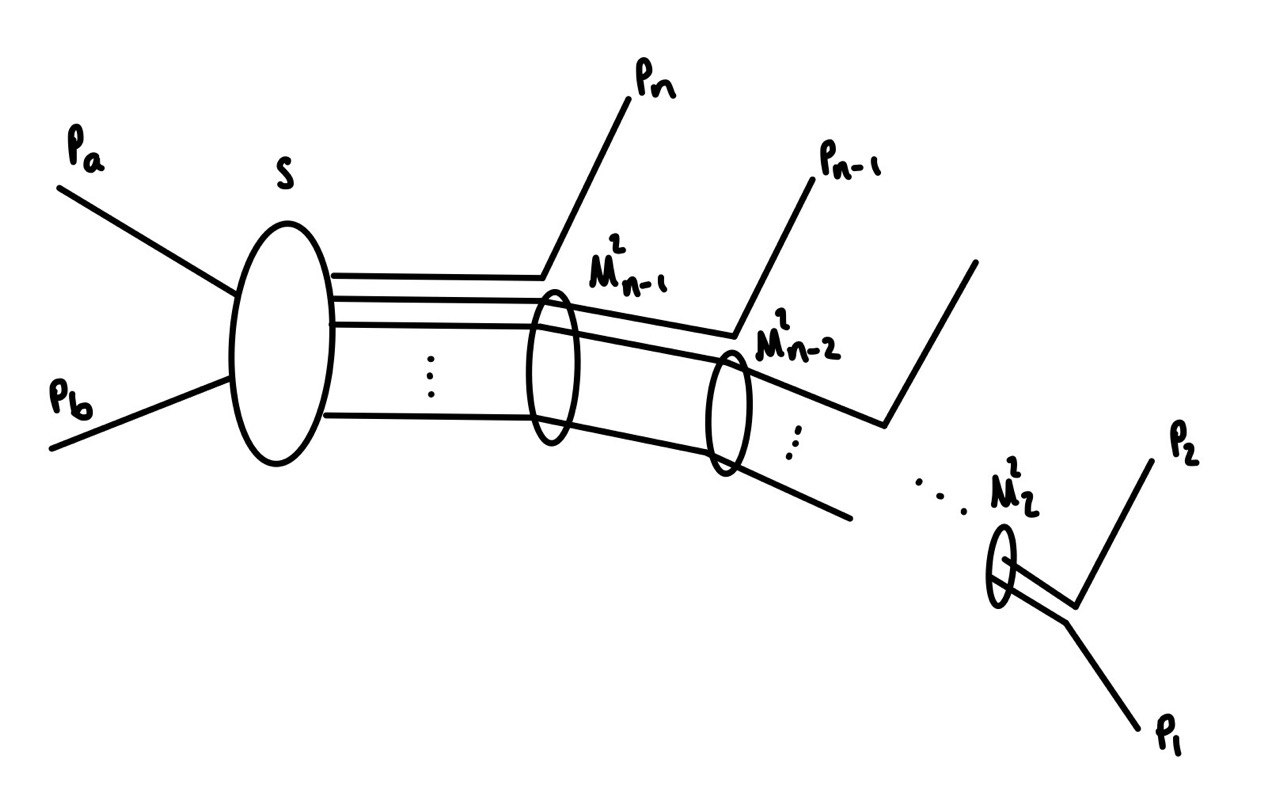
\includegraphics[width=0.6\linewidth]{figs/recursion-diagram.jpg}
    \caption{Illustration of the recursion relation as a sequence of effective $2 \rightarrow 2$ scattering events (this diagram is largely based on pg. 26 of \cite{James:1968gu}).}
    \label{fig:recursion-diagram}
\end{figure}

%====
% SUBSECTION: Writing the integral in terms of momentum transfers 
%====
\subsec{Writing integral in terms of momentum transfers}
\label{subsec:momentum-transfers}

In sec~\ref{subsec:recursive-relation} we wrote the phase space integral in terms of invariant masses and angles of the three-momenta $\bm{p}_i$ defined in the center-of-mass frame where $\sum_{k=1}^{i} p_k = (M_{i}, \bm{0})$. 
The matrix element in \eref{eq:matrix-element} is a function of the Lorentz invariants $(p_a \cdot p_1), \; (p_b \cdot p_3), \; (p_2 \cdot p_3)$, and $(p_b \cdot p_2) = (- (p_a - p_1 - p_2 - p_3) \cdot p_2)$. 
It is cumbersome to write this matrix element explicitly in terms of the angles $\{ (\theta_i, \varphi_i) : i = 1, 2, \ldots, n\}$ so we would rather use kinematic Lorentz invariants analogous to the Mandelstam variables for $2 \rightarrow 2$ scattering\footnotemark.
To this end it is convenient to introduce the so-called `momentum transfers' $t_i \equiv Q_i^2 \equiv (p_a - p_1 - \cdots - p_i)^2 = (p_n + p_{n-1} + \cdots + p_{i + 1} - p_b)^2$.

\footnotetext{At least, I think that is the motivation for introducing these variables.}

Some of the dot products (but not all) may be written exclusively in terms of the kinematic variables. For example,
\begin{gather*}
    \begin{align*}
        t_1 &\equiv (p_a - p_1)^2 &&\rightarrow 
        && 2 p_a \cdot p_1 = m_a^2 +  m_1^2 - t_1 \\
        t_2 &\equiv (p_a - (p_1 + p_2))^2 &&\rightarrow 
        && 2 p_a \cdot p_2 = M_2^2 - m_1^2 + t_1 - t_2 \\
        t_3 &\equiv (p_a - (p_1 + p_2 + p_3))^2 &&\rightarrow 
        && 2 p_a \cdot p_3 = M_3^2 - M_2^2 + t_2 \\
        M_2^2 &\equiv (p_1 + p_2)^2 &&\rightarrow 
        && 2 p_1 \cdot p_2 = M_2^2 - m_1^2 - m_2^2 \\
        M_3^2 &\equiv (p_1 + p_2 + p_3)^2 &&\rightarrow 
        && 2 (p_1 + p_2) \cdot p_3 = M_3^2 - 2 M_2^2 + m_1^2 + m_2^2 - m_3^2 
    \end{align*}\\
    2 p_b \cdot p_3 = 2 (p_1 + p_2) \cdot p_3 + 2 m_3^2  - 2 p_a \cdot p_3 =
    m_1^2 + m_2^2 + m_3^2 - M_2^2 - t_2
\end{gather*}
However I was unable to write $p_2 \cdot p_3$ in terms of the invariants alone. 
$p_b \cdot p_2$ is really just $p_2 \cdot p_3$ in disguise so it has the same problem.
I believe this is because these variables are not enough to fully describe the system and some angles are required in addition. 
We need $3(3) - 4 = 5$ integration variables but only $3$ of them are prescribed by the kinematic invariants $M_2^2$, $t_1$, and $t_2$\footnotemark.
I haven't followed their derivation through in enough detail to understand precisely how they show up in the expression 
\todo{
    Understand how to write the matrix element explicitly in terms of the angles $\varphi_1$, $\varphi_2$ as well as the invariants $M_2^2$, $t_1$, and $t_2$.
}.

The two additional degrees of freedom can be seen in eq. (14) of~\cite{Byckling:1969sx}. 
They are the azimuthal angles $\varphi_1$, $\varphi_2$ as seen in a frame where $p_a = (m_a, \bm{0})$.   

\footnotetext{$M_1^2 = m_1^2$,  $M_3^2 = s$ and  $t_3 = (-p_b)^2 = m_b^2$ are all constants, not integration variables.}  
    %====
% SECTION: Monte Carlo Integration
%====
\section{Monte Carlo integration}\label{sec:monte-carlo-integration}

%===
% SUBSEC: Introduction
%===
\subsection{The basics}\label{subsec:mc-basics}
Suppose you are interested in evaluating the integral 
\begin{align}
    I = \int_a^b f(x) \, \dd x.
\end{align}
The most obvious method of approximating this is with a Riemann sum or trapezoidal integration where you divide the domain into bins of width $\Delta x$ and calculate the area of a rectangle or trapezoid using the values of $f$ at the bin edges. 

Monte Carlo integration, on the other hand, takes a a different approach altogether whereby points in the domain are sampled at random and the integral is approximated as an average. 
To see this, note that the average value of $f$ on the domain is
\begin{align}
    \langle f \rangle = \frac{1}{b - a} \int_a^b f(x)\, \dd x = \frac{I}{b - a}.
\end{align}
The average $\langle f \rangle$ can be approximated by uniformly sampling $N$ i.i.d random numbers $x_i$ on the domain $x \in [a, b]$ where $i \in {1, 2, ..., N}$ and calculating the mean of $f(x_i)$:
\begin{align}
    \langle f \rangle \approx \langle f \rangle_N \equiv \frac{1}{N}\sum_{i = 1}^{N} f(x_i).
\end{align}
Therefore we can approximate the integral $I$ as
\begin{align}
    I \approx (b - a) \langle f \rangle_N.
\end{align}
This argument can be extended to higher dimensions, i.e. in $n$ dimensions we have
\begin{align}
    I = \int_V f(\bm{x}) \, \dd^n x = V \langle f \rangle.
\end{align}
One important result is that this strategy always converges as $N^{-1/2}$ in all dimensions, whereas techniques like trapezoidal integration converge rapidly in one dimension ($N^{-2}$), but significantly slower for higher dimensions ($N^{-2/n}$). For example in 5 dimensions, trapezoidal integration converges like  $N^{-2/5}$, which is slower than Monte Carlo integration.

%===
% SUBSEC: Importance sampling
%===
\subsec{Importance sampling}
\label{subsec:mc-importance-sampling}
In sec. \ref{subsec:mc-basics} we sampled $x$ uniformly at random on the domain of integration. However, we can choose to sample $x$ from any arbitrary distribution $p(x)$ and compute the same expectation value by weighting the sample $f(x)$ by $1 / p(x)$ so that
\begin{align}
    I \approx \frac{V}{N}\sum_{i=1}^{N} \frac{f(x_i)}{p(x_i)}.
\end{align}
With an appropriate choice of $p$ our Monte Carlo integration technique can be made to converge significantly faster than by sampling $x$ uniformly at random. 
To see why this is, suppose $f(x) = e^{-x^2}$ and $[a,b] = [-1000, 1000]$. 
Sampling uniformly on $[-1000, 1000]$ means that the majority of points we pick will be in the tails of the Gaussian and will hardly affect the value of the integral. 
If instead we sampled from a standard normal distribution we would mostly choose $x$ values near the peak at $x = 0$ and our result would converge much more rapidly.
Clearly the choice of $p$ is heavily dependent on the particular shape of the integrand $f$. 
\hl{The Metropolis-Hastings algorithm is one way to generate samples $x$ from $p(x)$ and can be used for importance sampling.}

\underline{VEGAS algorithm:}

The discussion of the VEGAS algorithm at \url{https://www.ippp.dur.ac.uk/~krauss/Lectures/QuarksLeptons/Basics/PS_Vegas.html} is quite good. In case the link breaks in the future I reproduce some of the main points below.
\begin{quotation}
    ``The VEGAS algorithm starts by dividing the $n$-dimensional hypercube $[0,1]^n$ into smaller ones -- usually of identical size -- and performs a sampling in each of them. 
    The results are then used to refine the integration grid for the next iteration of the sampling procedure.''
\end{quotation}
 
\subsec{Stratified sampling}
\label{subsec:stratified-sampling}

\subsec{Multichannel sampling}
\label{subsec:multichannel-sampling}


    \section{Tackling a simpler integral}
\label{sec:a-simpler-integral}
\hl{August 28 2023:} I spent the last week working on the response to the referee on my non-Gaussianity from axion-string birefringence paper. 
Now I want to return to this integral project.

I will try doing a simpler integral where the ingoing particle momenta $p_a$ and $p_b$ are fixed and we integrate only over the outgoing states. 
I will also drop the Lorentz-invariance breaking thermal factors. 
\begin{align}
    \int \sum_{\sigma, \sigma'} | \mathcal{M} |^2 \dd \Phi_3(s)
\end{align}

I will take 
\begin{align}
    m_a &= m_e = 0.5 \ \mathrm{MeV} \\
    m_b &= m_p = 938.272 \ \mathrm{MeV} \\
    m_1 &= m_\mu = 106 \ \mathrm{MeV} \\
    m_2 &= 0 \\
    m_3 &= 0
\end{align}
and 
\begin{align}
    p_a &= (m_a, \bm{0}) \\
    p_b &= (E_b, \bm{p}_b), \ \bm{p}_b = \bm{i} + \bm{j} + \bm{k}, \ E_b = \sqrt{|\pvec[b]|^2 + m_b^2}\ . 
\end{align}

%=====
% SUBSECTION: Integrating directly over C.o.M. energies
%=====
\subsec{Integrating directly over CM energies}
\label{subsec:simple-integral-CM-energies}

%=====
In this section I describe a technique for performing phase space integrals directly in terms of the variables $E_1,\, E_2,\, \varphi_{12},\, \cos\theta_{1},$ and $\varphi_{1}$ where all quantities are in the center of mass (CM) frame of the incident particles, $\pvec[a] + \pvec[b] = 0$. 

Consider the LIPS measure for 3 outgoing particles
\begin{align}
    \dd \Phi_3 (s) = 
    (2\pi)^{-5}
    \delta^4(p_a + p_b - p_1 - p_2 - p_3)
    \, \frac{\dd^3 p_1}{2 E_1} 
    \, \frac{\dd^3 p_2}{2 E_2}
    \, \frac{\dd^3 p_3}{2 E_3} \ .
\end{align}
We can use the momentum-conserving $\delta$-function to evaluate the $\dd^3 p_3$ integral so that in the CM frame we have
\begin{align}
    \dd \Phi_3 (s) \rightarrow
    (2\pi)^{-5}
    \delta(\sqrt{s} - E_1 - E_2 - E_3)
    \, \frac{1}{2 E_3} 
    \, \frac{\dd^3 p_1}{2 E_1} 
    \, \frac{\dd^3 p_2}{2 E_2} \ ,
\end{align}
where in the above expression it is understood that $E_3$ is to be replaced with $\sqrt{(-\pvec[1] - \pvec[2])^2 + m_3^2}$.
Now rewrite the $\dd^3 p_i$ integrals in spherical polar coordinates, 
\begin{align}
    \dd \Phi_3 (s) \rightarrow
    (2\pi)^{-5}
    \delta(\sqrt{s} - E_1 - E_2 - E_3)
    \, \frac{1}{2 E_3} 
    \, \frac{|\pvec[1]|^2 \dd |\pvec[1]| \, \dd \cos \theta_1 \, \dd \varphi_1}{2 E_1} 
    \, \frac{|\pvec[2]|^2 \dd |\pvec[2]| \, \dd \cos \theta_{12} \, \dd \varphi_{12}}{2 E_2} \ .
\end{align}
$(\theta_{1}, \varphi_{1})$ give the polar and azimuthal angles of $\pvec[1]$ in the CM frame, whereas $(\theta_{12}, \varphi_{12})$ give the polar and azimuthal angles of $\pvec[2]$ relative to $\pvec[1]$. 
This means that $\varphi_1$ and $\varphi_{12}$ are not measured in the same plane (unless $\theta_1 = 0$).
We use the energy-conserving Dirac delta to evaluate the $\dd \cos \theta_{12}$ integral, obtaining
\begin{align}
    &\cos \theta_{12} =
    \frac{s + 2 E_1 E_2 - 2 \sqrt{s}(E_1 + E_2) + m_1^2 + m_2^2 - m_3^2}{2 \sqrt{E_1^2 - m_1^2} \, \sqrt{E_2^2 - m_2^2}} \  , \\
    &\frac{\dd}{\dd \cos\theta_{12}} (\sqrt{s} - E_1 - E_2 - E_3) = - \frac{2 |\pvec[1]| |\pvec[2]|}{E_3} \ , 
\end{align} 
so that the $\dd \cos \theta_{12}$ integral can be done by making the replacement $\delta(\sqrt{s} - E_1 - E_2 - E_3) \, \dd \cos \theta_{12} \rightarrow E_3 / (2 |\pvec[1]| |\pvec[2]|)$.
Hence,
\begin{equation}
    \dd \Phi_3 (s) \rightarrow 
    \frac{(2\pi)^{-5}}{2^3 E_1 E_2 E_3} 
    \, \frac{E_3}{2 |\pvec[1]| |\pvec[2]|} 
    \, |\pvec[1]|^2 |\pvec[2]|^2
    \, \dd |\pvec[1]| \, \dd |\pvec[2]| 
    \, \dd \cos \theta_1 \, \dd \varphi_1 
    \, \dd \varphi_{12} \ .
\end{equation}
We also have 
\begin{align}
    |\pvec[i]|^2 = E_i^2 - m_i^2  \Rightarrow  |\pvec[i]| \dd |\pvec[i]| =  E_i \dd E_i \ , 
\end{align}
and so
\begin{equation}
    \dd \Phi_3 (s) \rightarrow 
    \frac{(2\pi)^{-5}}{2^3} 
    \, \dd E_1 \, \dd E_2 
    \, \dd \cos \theta_1 \, \dd \varphi_1 
    \, \dd \varphi_{12} \ .
\end{equation}
To obtain the limits of integration I found that it's actually easier to introduce the kinematic Lorentz invariants
\begin{align}
    s_1 &= (p_a + p_b - p_1)^2 = (p_2 + p_3)^2 \\
    s_2 &= (p_a + p_b - p_2)^2 = (p_3 + p_1)^2 \\
    s_3 &= (p_a + p_b - p_3)^2 = (p_1 + p_2)^2
\end{align}
which are related to the CM frame energies by $E_i = (s + m_1^2 - s_i)/2 \sqrt{s}$. 
The $s_i$ are not independent and satisfy $s_1 + s_2 + s_3 = s + m_1^2 + m_2^2 + m_3^2$. 
This excercise is done in detail in~\url{https://web.physics.utah.edu/~jui/5110/hw/kin_rel.pdf}. 
The key results are as follows. 
If none of the $s_i$ are fixed then $s_1 \in [(m_2 + m_3)^2, (\sqrt{s} - m_1)^2]$.
If $s_1$ is picked from that interval then $s_2$ is bounded by 
\begin{align}
    \label{eq:s2-bounds}
    s_2^{\pm} = m_1^2 + m_3^2 + \frac{1}{2 s_1} 
    \left[
        (s - s_1 - m_1^2)(s_1 - m_2^2 + m_3^2) \pm \sqrt{\lambda(s_1, s, m_1^2) \lambda(s_1, m_2^2, m_3^2) }
    \right] \ .
\end{align}
Therefore to sample $(E_1, E_2, \cos \theta_1, \varphi_1, \varphi_{12})$ from the kinematically allowed region of phase space one may make use of the following procedure.
\begin{enumerate}
    \item Draw $E_1$ uniformly at random from the interval $[m_1, (s + m_1^2 - (m_2 + m_3)^2) / 2 \sqrt{s}]$. 
    \item Draw $E_2$ uniformly at random from the interval $[\frac{s + m_2^2 - s_2^{+}}{2 \sqrt{s}}, \frac{s + m_2^2 - s_2^{-}}{2 \sqrt{s}}]$, where $s_2^{\pm}$ is given by~\eref{eq:s2-bounds} and $s_1$ takes the value generated in step 1.
    \item Draw $\cos \theta_1$ uniformly from $[-1, 1]$.
    \item Independently draw $\varphi_1$ and $\varphi_{12}$ uniformly from $[0, 2\pi]$. 
\end{enumerate}
The CM frame momentum vectors for the outgoing particles may then be reconstructed as
\begin{align}
    \pvec[1] &= \sqrt{E_1^2 - m_1^2} 
    (\sin \theta_1 \cos\varphi_1 \mathbf{i} 
    + \sin \theta_1 \, \sin\varphi_1 \mathbf{j} 
    + \cos\theta_1 \mathbf{k}) \\
    \pvec[2] &= \sqrt{E_2^2 - m_2^2} \, R^{-1}_{\theta_1, \varphi_1} 
    (\sin \theta_{12} \cos\varphi_{12} \mathbf{i} 
    + \sin \theta_{12} \, \sin\varphi_{12} \mathbf{j} 
    + \cos\theta_{12} \mathbf{k}) \\
    \pvec[3] &= - \pvec[1] - \pvec[2] \ ,
\end{align}
where $\sin \theta$ is given by$\sqrt{1 - \cos \theta^2}$ and $R_{\theta, \varphi}$ is a rotation matrix that takes $\mathbf{k}$ into the $(\theta, \varphi)$ direction (in particular, I used \texttt{R[theta\_, phi\_] := EulerMatrix[\{phi, theta, 0\}]}). 

%====
% SUBSECTION: Intermediate results
%====
\subsec{Preliminary results}
\label{subsec:preliminary-results}

%====
% PHASE SPACE VOLUME 
%====
\subsubsection*{Phase space volume}
The first check I did was to make sure that the phase space volume given by $\mathcal{I} = \int \dd \Phi_3(s)$ is the same for both techniques. 
I calculated the phase space volume using the methods described in~\sref{subsec:simple-integral-CM-energies} and~\sref{subsec:momentum-transfers}.
Performing a Monte Carlo integration over the energies as in~\sref{subsec:momentum-transfers} with chains of length $N = 100,000$, gave \hl{$\mathcal{I}_{\mathrm{Energy}} = 98.7 \pm 0.13$}. 
The error is calculated as the standard deviation from 10 independent runs of the integration method. 
The central value is the mean of the ten chains. 
It took \hl{35 seconds} to run the ten chains for this method.
Meanwhile doing the Monte Carlo integration using the momentum transfer technique as in~\sref{subsec:simple-integral-CM-energies} gave 
\hl{$\mathcal{I}_{\mathrm{mom. trans.}} = 98.7 \pm 0.15$}.
It took \hl{$60$ seconds} to run the ten chains for this method.
I also verified that the variance goes as $N^{-1/2}$, as expected for Monte Carlo integration.

%====
% INTEGRAL OVER THE MATRIX ELEMENT
%====
\subsubsection*{$\overline{|\mathcal{M}|^2}$ integral}
The second test I did was to integrate the spin-summed squared matrix element over the outgoing particles,
\begin{align}
    \int \overline{|\mathcal{M}|^2} \, \dd \Phi_3 (s) \ .
\end{align}
Below are the results for $N = 100,000$, using 10 runs to estimate the standard deviation:\\\\
\hl{{\underline{Energy method:}}
$(1.92 \pm 0.03) \times 10^{-2}$.
Took $340$ seconds.}\\\\
\hl{{\underline{Momentum transfer method:}}
$(2.00 \pm 0.02) \times 10^{-2}$. 
Took $51$ seconds.}

They converge to different central values but they are still `close' with an error of $\sim 4\%$. 

%====
% INTEGRAL OVER THE MATRIX ELEMENT
%====
\subsubsection*{$E_3$ integral}
The third test I did was to integrate the outgoing axion neutron-star-rest-frame energy, $E_3$
\begin{align}
    \int E_3 \, \dd \Phi_3 (s) \ .
\end{align}

    % %====
% % SECTION: SOFTWARE PACKAGES 
% %====
% \section{CompHEP and MADGRAPH5}
% \label{sec:software}

% %----
% % SUBSECTION: CompHEP
% %----
% \subsec{\code{CompHEP}}
% \label{subsec:comphep}
% \newcommand{\comphep}[1][]{\code{CompHEP}}
% While I was looking for ways to do the integral I found a software called \comphep~\cite{Boos:1994xb} which does a lot of the things I am interested in doing. 
% \comphep is a ``a package for evaluation of Feynman diagrams, integration over multi-particle phase space and event generation''. 
% It allows the user to specify a Lagrangian and then it can generate tree level Feynman diagrams for a user-specified process, along with C and Fortran code to evaluate matrix elements. 
% It can even compute cross-sections/other observables.
% \comphep has two main backbones: (i) symbolic calculations (ii) numerical calculations.

% The main tasks performed by the symbolic part are
% \begin{enumerate}[itemsep=-2ex]
%     \item Select a process by specifying in and out states for decays into up to $5$ outgoing particles or collisions of $2 \rightarrow 2, \  2 \rightarrow 3, \  2 \rightarrow 4$.
%     \item Generate Feynman diagrams.
%     \item Delete unwanted diagrams.
%     \item Compute S-matrix elements.
%     \item Save symbolic results so they can be further analysed in \code{Mathematica}.
%     \item Generate C and Fortran code for the matrix elements to be used in numerical studies.
% \end{enumerate}

% The numerical part, on the other hand, performs Monte Carlo integration and event generation. 
% The main tasks performed are:
% \begin{enumerate}[itemsep=-2ex]
%     \item Choose phase space kinematic variables (\hl{idk what this means yet})
%     \item Introduce kinematic cuts over squared momentum transfers (\hl{not sure what the significance of this is})
%     \item Perform regularization to remove sharp peaks in matrix elements.
%     \item Calculate distributions, cross-sections, or particle width using Monte Carlo methods.
%     \item Perform integration, taking into account structure functions for ingoing particles.
%     \item Event generation.
% \end{enumerate}


    \appendix

%====
% Appendix A: Derivation of the recursive relation in eq:recursive-phase-space-relation
%====
\section{Derivation of recursive relation}
This appendix fills in the details for the derivation of eq. (\ref{eq:recursive-phase-space-relation}) which are left out in~\cite{Byckling:1969sx}. Our starting point is 
\begin{align*}
    R_n(s) 
        &= 
        \int \prod_{i=1}^{n} \delta (p_i^2 - m_i^2) \, \Theta(p_i^0) \, 
        \dd^4 p_i \, \delta^4(p_a + p_b - p_1 - \cdots - p_n) \\
        &=
        \int
        \delta(p_n^2 - m_n^2) \, \Theta(p_n^0) \, \dd^4 p_n 
        \bigg[
            \prod_{i=1}^{n-1} 
            \delta (p_i^2 - m_i^2) \, \Theta(p_i^0)
        \bigg]
        \delta^4(p_a +  p_b - p_n - p_1 - \cdots - p_{n-1}) \\
        &=
        \int
        \delta(p_n^2 - m_n^2) \, \Theta(p_n^0) \, \dd^4 p_n \, 
        R_{n-1}(p_a + p_b - p_n)
\end{align*}
Multiply the RHS by $\int \dd M_{n-1}^2\,\delta(M_{n-1}^2 - (p_a + p_b - p_n)^2)$. 
\begin{align*}
    \int \dd M_{n-1}^2 \, \delta\big(M_{n-1}^2 - (p_a + p_b - p_n)^2\big) \,
    \delta(p_n^2 - m_n^2) \, \Theta(p_n^0) \, \dd^4 p_n \,
    R_{n-1}\big(p_a + p_b - p_n\big).
\end{align*}
Use the on-shell delta function to do the $p_n^0$ integral and write $\dd^3 p_n$ in terms of spherical coordinates:
\begin{align*}
    &\int \dd M_{n-1}^2 \, \delta\big(M_{n-1}^2 - (p_a + p_b - p_n)^2\big) \,
    \, \frac{\dd^3 p_n}{2 E_n} \,
    R_{n-1}\big(p_a + p_b - p_n\big)\\
    &= 
    \int \dd M_{n-1}^2 \, \delta\big(M_{n-1}^2 - (p_a + p_b - p_n)^2\big) \,
    \, \frac{|\bm{p}_n|^2 \dd |\bm{p}_n| \dd \Omega_n}{2 E_n} \,
    R_{n-1}\big(p_a + p_b - p_n\big).
\end{align*}
Then use the $M_{n-1}^2$ Dirac delta to do the $\dd |\bm{p}_n|$ integral. 
This requires us to (i) solve $M_{n-1}^2 - (p_a + p_b - p_n)^2 = 0$ for $|\bm{p}_n|$; (ii) evaluate $\dd / \dd |\bm{p}_n| \big(M_{n-1}^2 - (p_a + p_b - p_n)^2\big)$; and (iii) impose $|\bm{p}_n|^2 \geq 0$ to derive bounds of integration for $\int \dd M_{n-1}^2$.
%===
% enumerate environment
%===
\begin{enumerate}[label=(\roman*)]
    %----
    % (i) Solving for |p_n|
    %----
    \item We start by expanding the LHS
    \begin{align*}
        &M_{n-1}^2 - (p_a + p_b - p_n)^2 = M_{n-1}^2 - (p_a + p_b)^2 - p_n^2 + 2(p_a + p_b) \cdot p_n \\
        &= M_{n-1}^2 - s - m_n^2 + 2 (E_a + E_b) E_n + 2 (\bm{p}_a + \bm{p}_b) \cdot \bm{p}_n.
    \end{align*}
    Now we choose the center of mass frame so that $\bm{p}_a + \bm{p}_b = 0$. This is valid because the integral is a Lorentz invariant, so the final result is independent of the reference frame. 
    \begin{align*}
        &M_{n-1}^2 - s - m_n^2 + 2 (E_a + E_b) E_n + 2 (\bm{p}_a + \bm{p}_b) \cdot \bm{p}_n\\
        &=
        M_{n-1}^2 - s - m_n^2 + 2 \, \sqrt{s} \, \sqrt{|\bm{p}_n|^2 + m_n^2} = 0.
    \end{align*}
    Now we can rearrange and solve for $|\bm{p}_n|$
    \begin{align*}
        |\bm{p}_n|^2 
        &=
        \frac{(s + m_n^2 - M_{n-1}^2)^2}{4 s} - m_n^2 = 
        \frac{s^2 + m_n^4 + M_{n-1}^4 - 2 s m_n^2 - 2 s M_{n-1}^2 - 2 m_n^2 M_{n-1}^2}{4 s} \\
        &\equiv \boxed{\frac{\lambda(s, M_{n-1}^2, m_n^2)}{4s}}\;.
    \end{align*}
    $\lambda(x,y,z) = x^2 + y^2 + z^2 - 2xy - 2xz - 2yz$ is called the \href{https://en.wikipedia.org/wiki/K%C3%A4ll%C3%A9n_function}{K\"{a}llen function}.
    %----
    % (ii) Evaluating a derivative
    %----
    \item%
    \begin{align*}
        &\frac{\dd}{\dd |\bm{p}_n|} 
        \bigg( 
            M_{n-1}^2 - (p_a + p_b - p_n)^2
        \bigg)\\
        &= 
        \frac{\dd}{\dd |\bm{p}_n|} 
        \bigg( 
            M_{n-1}^2 - s - m_n^2 + 2 \, \sqrt{s} \, \sqrt{|\bm{p}_n|^2 + m_n^2}
        \bigg)\\
        &=
        \boxed{\frac{2\sqrt{s}\,|\bm{p}_n|}{E_n}}
    \end{align*}
    %----
    % (iii) Getting upper bound of integration by imposing |p_n| > 0
    %----
    \item%
    \begin{align*}
        &|\bm{p}_n|^2 \geq 0 \\
        &\Rightarrow \lambda(s, M_{n-1}^2, m_n^2) \geq 0\\
        &\Rightarrow 
        \big[
            M_{n-1}^2 - (s + m_n^2)
        \big]^2
        - 4\,s m_n^2
        \geq 0\\
        &\Rightarrow
        \big[
            M_{n-1}^2 - (s + m_n^2)
        \big]^2
        \geq 4\,s m_n^2\\
        &\Rightarrow
            M_{n-1}^2 - (s + m_n^2) \geq 2 \sqrt{s\, m_n^2} 
            \; \big|\big| \;
            M_{n-1}^2 - (s + m_n^2) \leq - 2 \sqrt{s\, m_n^2}  \\
            &\Rightarrow
            M_{n-1}^2 \geq (s + m_n^2) + 2 \sqrt{s\, m_n^2} 
            \; \big|\big| \;
            M_{n-1}^2 \leq (s + m_n^2) - 2 \sqrt{s\, m_n^2}  \\
            &\Rightarrow
            \boxed{
                M_{n-1}^2 \geq (\sqrt{s} + m_n)^2
                \; \big|\big| \;
                M_{n-1}^2 \leq (\sqrt{s} - m_n)^2.
            }
    \end{align*}
    
\end{enumerate}
With these results established we find that 
\begin{align}
    \delta \big( M_{n-1}^2 - (p_a + p_b - p_n)^2 \big)
    = \frac{
        \delta \Big(
        |\bm{p}_n| - \sqrt{\lambda(s, M_{n-1}^2, m_n^2)} \Big/ (2 \sqrt{s})    
    \Big)
    }
    {
        2 \sqrt{s}\, |\bm{p}_n| / E_n
    }\;\;.
\end{align}
Hence,
\begin{align*}
    &\int \dd M_{n-1}^2 \, \delta\big(M_{n-1}^2 - (p_a + p_b - p_n)^2\big) \,
    \, \frac{|\bm{p}_n|^2 \dd |\bm{p}_n| \dd \Omega_n}{2 E_n} \,
    R_{n-1}\big(p_a + p_b - p_n\big)\\
    &= 
    \int \dd M_{n-1}^2 \, 
    \frac{
        \delta \Big(
        |\bm{p}_n| - \sqrt{\lambda(s, M_{n-1}^2, m_n^2)} \Big/ (2 \sqrt{s})    
    \Big)
    }
    {
        2 \sqrt{s}\, |\bm{p}_n| / E_n
    }
    \,
    \, \frac{|\bm{p}_n|^2 \dd |\bm{p}_n| \dd \Omega_n}{2 E_n} \,
    R_{n-1}\big(p_a + p_b - p_n\big) \\
    &=
    \int \dd M_{n-1}^2 \, 
    \frac{\sqrt{\lambda(s, M_{n-1}^2, m_n^2)}}{8 s}
    \, \dd \Omega_n \,
    R_{n-1}\big(M_{n-1}^2).
\end{align*}

    % end notes
\bibliography{ref}
\bibliographystyle{unsrt}
\end{document}